\documentclass{article}

\usepackage{fancyhdr}
\usepackage{extramarks}
\usepackage{amsmath}
\usepackage{amsthm}
\usepackage{amsfonts}
\usepackage{tikz}
\usepackage[plain]{algorithm}

\usetikzlibrary{automata,positioning}
\usepackage{titling}
\usepackage{chngcntr}
\counterwithin{figure}{section}
\usepackage{sectsty}
\sectionfont{\fontsize{15}{15}\selectfont}
\usepackage{multirow}
\usepackage{booktabs}
\usepackage{arydshln}
\usepackage[font={scriptsize}]{caption}
\usepackage{listings}
\usepackage{color}
\definecolor{mygreen}{RGB}{28,172,0} 
\definecolor{mylilas}{RGB}{170,55,241}
%
% Basic Document Settings
%

\topmargin=-0.45in
\evensidemargin=0in
\oddsidemargin=0in
\textwidth=6.5in
\textheight=9.0in
\headsep=0.25in

\linespread{1.1}

\pagestyle{fancy}
\lhead{\hmwkClass}
\rhead{\hmwkTitle}
\cfoot{\thepage}

\renewcommand\headrulewidth{0.4pt}
\renewcommand\footrulewidth{0.4pt}
\renewcommand{\thesubsubsection}{\alph{subsubsection})}
\setlength\parindent{0pt}

\lstdefinestyle{matlab}{
	language=Matlab,%
    basicstyle=\scriptsize,
    breaklines=true,%
    morekeywords={matlab2tikz},
    keywordstyle=\color{blue},%
    morekeywords=[2]{1}, keywordstyle=[2]{\color{black}},
    identifierstyle=\color{black},%
    stringstyle=\color{mylilas},
    commentstyle=\color{mygreen},%
    showstringspaces=false,%without this there will be a symbol in the places where there is a space
    %numbers=left,%
    %numberstyle={\tiny \color{black}},% size of the numbers
    %numbersep=9pt, % this defines how far the numbers are from the text
    emph=[1]{for,end,break},emphstyle=[1]\color{red}, %some words to emphasise
    %emph=[2]{word1,word2}, emphstyle=[2]{style},    
}
%
% Homework Details
%   - Title
%   - Due date
%   - Class
%   - Section/Time
%   - Instructor
%   - Author
%

\newcommand{\hmwkTitle}{}
\newcommand{\hmwkDueDate}{}
\newcommand{\hmwkClass}{Lyapunov function based control of a Type-(1,1) Robot  \\without using the reference steering angle}
\newcommand{\hmwkClassTime}{}
\newcommand{\hmwkClassInstructor}{}
\newcommand{\hmwkAuthorName}{}
\newcommand{\hmwkAuthorEmail}{Subodh.Mishra.eleves@ec-nantes.fr}
\newcommand{\figurescaling}{width=\textwidth}


\begin{document}
\clearpage
\thispagestyle{empty}
\clearpage
\noindent\rule{\textwidth}{0.4pt} \\
\textbf{\MakeUppercase{\hmwkClass}} \\
\textbf{\MakeUppercase{\hmwkTitle}} \\
\hmwkDueDate \\
Subodh Mishra\\
Truong Giang Vo
%-----------------------------------TOP PAGE-----------------------------

\noindent\rule{\textwidth}{0.4pt}
\section{Introduction}
A simplified figure of the type (1,1) wheeled mobile robot is presented below in Figure 1.1. $a$ is the distance between the wheel centre of the fixed wheels and the centre of steerable wheel. $\beta$ is the steering angle and $\theta$ is the orientation of the $R_m$ frame (also called the robot frame) with respect to the $R_O$ frame(the world frame). The objective is to design a controller based on a Lyapunov function to make the robot follow a circular trajectory of radius 2 metre and angular velocity 0.5 radian per second. In Figure 1.1, $R$ is the perpendicular distance of the instantaneous centre of rotation (ICR) from the centre (s) of the steerable wheel.
\begin{figure}[H]
\centering
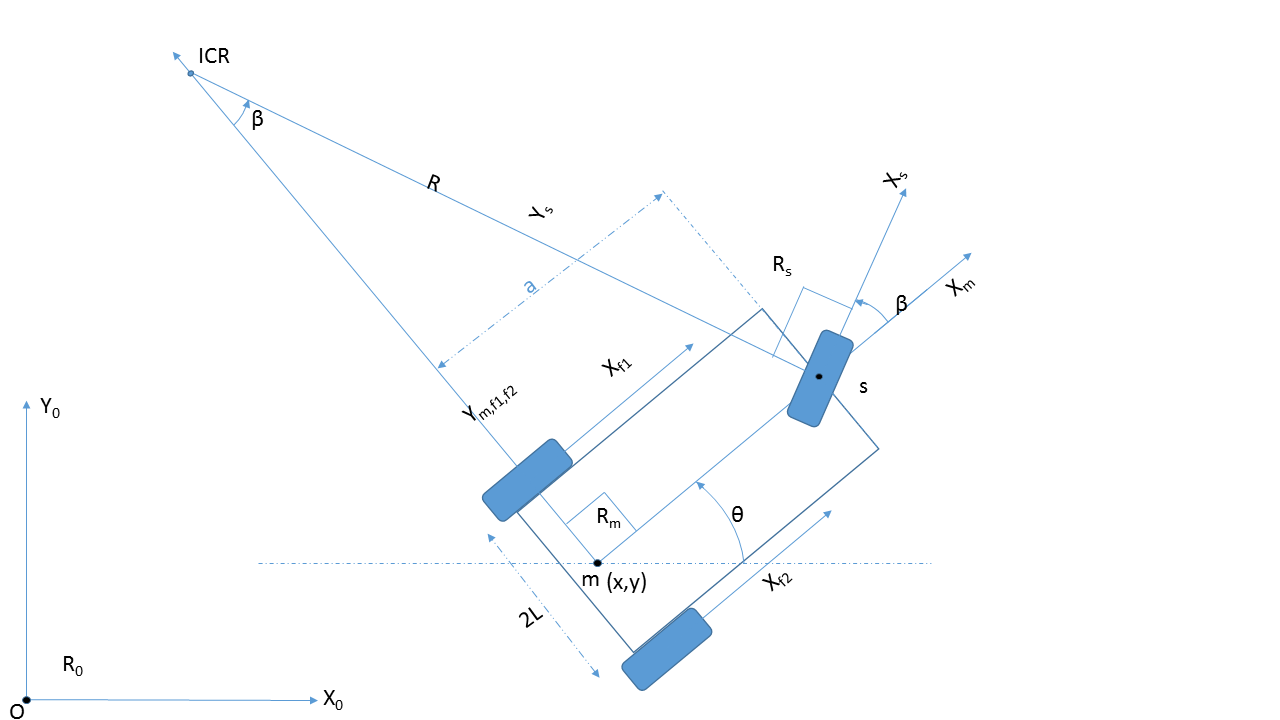
\includegraphics[width = 0.8\textwidth]{Figures/figure1.png}
\caption{Schematic of Type 11 Robot}
\label{fig:figure1}
\end{figure}
\section{The Posture Kinematic Model}
A possible kernel obtained from the matrix form of the no-skidding constraints for the type (1,1) wheeled mobile robot is:

\[\Sigma=
\begin{bmatrix}
    1\\
    0\\
    \frac{\tan \beta}{a} \\
\end{bmatrix}\]
Using the aforementioned kernel, the posture kinematic model of the type (1,1) robot is as follows:
\begin{align*} 
\dot{x}&=a\cos \theta u_m\\ 
\dot{y}&=a\sin \theta u_m\\
\dot{\theta}&=\frac{\tan \beta}{a}u_m\\
\dot{\beta}&=u_s
\end{align*}
Here, $u_m$ and $u_s$ are the inputs to the Posture Kinematic Model. While $u_s$ is the rate of change of orientation of the steering wheel, $u_m$ is the net translational velocity of the robot.  
\section{Configuration Kinematic Model and Wheel Motorization}
For the same kernel as discussed in the section 2, the complete Configuration Kinematic Model of the type (1,1) wheeled mobile robot is:

\[\begin{bmatrix}
\dot{x}\\
\dot{y}\\
\dot{\theta}\\
\dot{\beta}\\
\dot{\phi}_{f1}\\
\dot{\phi}_{f2}\\
\dot{\phi}_{s}\end{bmatrix}=\begin{bmatrix}
 a\cos \theta  & 0\\
 a\sin \theta  & 0\\
 \frac{\tan \beta}{a} & 0\\
 0 & 1\\
 \frac{1}{r}+\frac{L\tan \beta}{ar} & 0\\
 \frac{1}{r}-\frac{L\tan \beta}{ar}  & 0\\
 \frac{1}{r\cos \beta} & 0\end{bmatrix} \begin{bmatrix}
 u_m \\ u_s
 \end{bmatrix}\]
 Here $\dot{\phi}_{f1}$, $\dot{\phi}_{f2}$ and $\dot{\phi}_{s}$ are the angular velocities of the fixed wheels and the steerable wheel about their corresponding spin axes and $2L$ is the distance between the two fixed wheels(the origin of the robot frame,$R_m$, is at the centre of the common axle of the two fixed wheels).
 \subsection{Wheel Motorisation}
 The degree of mobility of the type (1,1) wheeled mobile robot is $\delta m=$ 1. Hence, only 1 out of the last three rows of the configuration kinematic models needs to be picked to complete the motorisation of this robot. Owing to mathematical simplicity and ease of inversion, the last row is chosen, which implies the spin of the steerable wheel about its y-axis is motorized. There is a singularity when $\beta m=\frac{\pi}{2}$, but this situation is highly unlikely and practically not allowed to occur. It should be noted that the steering joint (joint angle $\beta$), which gives the rotation of the steerable wheel about its z-axis, is also motorized, but this does not come under wheel spin motorisation. The wheel spin motorisation obtained is:
 $$\dot{\phi}_s=\frac{1}{r\cos \beta}u_m$$
The above equation is the inverse kinematic model.
\section{Theoritical study}
For the control design, let us consider two inputs, $u_m$ and a new input $u_{\omega}$. $u_{\omega}$ is actually the rate of change of orientation of the robot and in equation one can write:\\
 $$\dot{\theta}=u_{\omega}= \frac{\tan \beta}{a}u_m$$
Using the above equation the steering angle can be found in terms of $u_m$ and $u_{\omega}$.
$$\beta= \tan^{-1}\bigg(\frac{au_{\omega}}{u_m}\bigg)$$
For tracking, the point $s$ is used. Point $s$ is the origin of the steerable wheel frame($R_s$,refer Figure 1.1). The orientation of the $R_m$ frame with respect to the 
$R_0$ frame is $\theta$. In the frame $R_0$, the posture to be tracked is:

\begin{align*} 
x_{s}&=x+a\cos \theta\\ 
y_{s}&=y+a\sin \theta\\
\theta&=\theta
\end{align*}

Here, (x,y) is the coordinate of the point $m$ in the $R_0$ frame. On taking the time derivative of the equations above, the following equation are obtained:\\
\begin{align*} 
\dot{x}_{s}&=\dot{x}-a\dot{\theta}\sin \theta \\ 
\dot{y}_{s}&=\dot{y}+a\dot{\theta}\cos \theta \\
\dot{\theta}&=\dot{\theta}
\end{align*}
Using the the posture kinematic model of section 2, the above equations can be written as:\\
\begin{align*} 
^{0}\dot{x}_{s}&=\cos \theta u_m - a\sin \theta u_\omega\\ 
^{0}\dot{y}_{s}&=\sin \theta u_m - a\cos \theta u_\omega\\ 
\dot{\theta}&=u_\omega
\end{align*}

$\implies$

\[\begin{bmatrix}
^{0}\dot{x}_{s}\\
^{0}\dot{y}_{s}\\
\dot{\theta}\end{bmatrix}=\begin{bmatrix}
\cos \theta & -a\sin \theta\\
\sin \theta &  a\cos \theta\\
0&1
 \end{bmatrix} \begin{bmatrix} u_m \\ u_{\omega} \end{bmatrix} \]
 
 This is the rate of change of state variables of the actual robot. Similarly, the virtual robot (the reference), which needs to be tracked (or followed) can be described by the following equations:
 
\[\begin{bmatrix}
^{0}\dot{x}_{sr}\\
^{0}\dot{y}_{sr}\\
\dot{\theta}_{r}\end{bmatrix}=\begin{bmatrix}
\cos \theta_r & -a\sin \theta_r\\
\sin \theta_r &  a\cos \theta_r\\
0&1
 \end{bmatrix} \begin{bmatrix} u_{mr} \\ u_{\omega r} \end{bmatrix} \]
 
All the state space equations developed above are with respect to the frame $R_0$.

Let error be defined as: $error=reference-actual$. In the $R_m$ frame, the errors in rate of change of $x$,$y$ and $\theta$ is:

\[\begin{bmatrix}
^{m}\dot{x}_{e}\\
^{m}\dot{y}_{e}\\
 \dot{\theta}_{e}\end{bmatrix}=\begin{bmatrix}
0\\
0\\
-\dot{\theta}
 \end{bmatrix} \times \begin{bmatrix} ^{m}x_{e}\\^{m}y_{e}\\\theta \end{bmatrix} + ^{m}\Omega_{0} (\theta)  \left[\begin{bmatrix} ^{0}\dot{x}_{sr}\\^{0}\dot{y}_{sr}\\ \dot{\theta}_{r} \end{bmatrix}-\begin{bmatrix} ^{0}\dot{x}_{s}\\^{0}\dot{y}_{s}\\ \dot{\theta} \end{bmatrix}\right]  \] 
 
Here, \[^{m}\Omega_{0}(\theta)=\begin{bmatrix}
\cos \theta & \sin \theta & 0\\
-\sin \theta& \cos \theta & 0\\
0&0&1 
\end{bmatrix}\] 
Using the equations developed in this section, the error model is simplified as:\\
\[\begin{bmatrix}
^{m}\dot{x}_{e}\\
^{m}\dot{y}_{e}\\
 \dot{\theta}_{e}\end{bmatrix}=\begin{bmatrix}
\cos \theta_e u_{mr}-a\sin \theta_e u_{\omega r}\\
\sin \theta_e u_{mr}+a\cos \theta_e u_{\omega r}\\
 u_{\omega r}
 \end{bmatrix}  +  \begin{bmatrix} -1 & ^{m}y_{e}\\
                                    0 &-(a+^{m}x_{e})\\
                                    0 & -1\end{bmatrix} \begin{bmatrix} u_{m} \\ u_{\omega} \end{bmatrix}  \] 
 
In short, the error model can be written as:
$\dot{X}=f(X,\textbf{u})$
Here, $X$ is the state variable vector and $\textbf{u}$ is the control input vector.
Consider a Lyapunov function $V(X)$ for the system $\dot{X}=f(X,\textbf{u})$. Designing a Lyapunov controller means finding a control input vector $\textbf{u}$ to satisfy:\\
$$\dot{V}(X)=\frac{\partial V}{\partial X}\dot{X}=\frac{\partial V}{\partial X}f(X,\textbf{u})<0$$
The Lyapunov function chosen must be positive definite. For this system, the Lyapunov function chosen is:
$$V(X)=\frac{1}{2}(^{s}x_{e}+^{s}y_{e}+\frac{^{s}\psi_{e}}{K_y})$$
$$\dot{V}(X)=\frac{\partial V}{\partial X}\dot{X}=\frac{\partial V}{\partial X}f(X,\textbf{u})<0$$
$\implies$
\[\begin{bmatrix}^{s}x_{e}&^{s}y_{e}&\frac{\psi_e}{K_y}\end{bmatrix}\begin{bmatrix}
^{s}\dot{x}_{e}\\
^{s}\dot{y}_{e}\\
 \dot{\psi}_{e}\end{bmatrix}<0\] 
 On simplifying:
 $$(\cos \theta_e u_{mr}-a\sin \theta_e u_{\omega r}-u_{mr})^{m}x_{e}+\bigg(\frac{\sin \theta_e u_{mr}+a\cos \theta_e u_{\omega r}}{\theta_e} ^{m}y_e+\frac{u_{\omega r}}{K_y}-(\frac{a ^{m}y_e }{\theta_e}+\frac{1}{K_y})u_{\omega}\bigg)\theta_{e}<0$$
 
 This inequality is satisfied if:
  \begin{align*}
\cos \theta_e u_{mr}-a\sin \theta_e u_{\omega r}-u_{m}&=-K_{x} ^mx_{e}\\
\bigg(\frac{\sin \theta_e u_{mr}+a\cos \theta_e u_{\omega r}}{\theta_e} ^{m}y_e+\frac{u_{\omega r}}{K_y}-(\frac{a ^{m}y_e }{\theta_e}+\frac{1}{K_y})u_{\omega}\bigg)&=-\frac{K_{\theta}}{K_{y}}\theta_{e}
 \end{align*}
 $\implies$
 \begin{align*}
u_{m}&=\cos \theta_e u_{mr}-a\sin \theta_e u_{\omega r}+K_{x} ^mx_{e}\\
u_{\omega}&=\frac{K_\theta \theta_e ^2 + u_{\omega r}\theta_e+K_y ^my_{e}(\sin \theta_e u_{mr}+a\cos \theta_e  u_{\omega r})}{K_y ^my_{e} a+\theta _e}
 \end{align*}
The above equations yield the value of the control inputs.\\
Hence,




\[\textbf{u}=\begin{bmatrix}
\cos \theta_e u_{mr}-a\sin \theta_e u_{\omega r}+K_{x} ^mx_{e}\\
\frac{K_\theta \theta_e ^2 + u_{\omega r}\theta_e+K_y ^my_{e}(\sin \theta_e u_{mr}+a\cos \theta_e  u_{\omega r})}{K_y ^my_{e} a+\theta _e}
 \end{bmatrix} \] 

The control objective is to force the robot to move along a circular trajectory centred at $(0,0)$ with radius $R=2$ m and angular velocity of $\omega_{d}=0.5$ rad/s, this implies that the tangential velocity of the robot must be $1$ m/s.\\

The translational velocity of the type (1,1) robot is $\dot{x}^{2}+\dot{y}^2=u_{m}$ must be equal to the tangential velocity required to satisfy the control objective. If the tangential velocity is $V_{tangential}$ then:
$$\dot{x}^{2}+\dot{y}^2=u_{m}=V_{tangential}$$

For the control objective specified, $V_{tangential}=R\omega_{d}=1$ m/s.
\section{Modelling}
\begin{figure}[H]
\centering
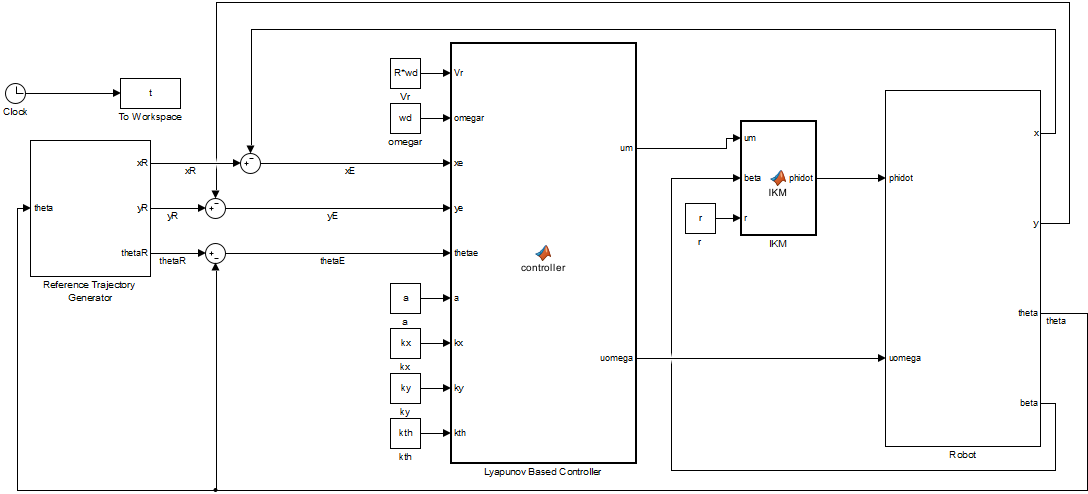
\includegraphics[width = 0.8\textwidth]{Figures/figure2.png}
\caption{Simulink Model of Lyapunov Controlled Type (1,1) Robot}
\label{fig:figure2}
\end{figure}

Figure \ref{fig:figure2} presents the \texttt{simulink} model of the Lyapunov function controlled Type(1,1) robot. A brief description of all the subsystems is presented below:\\

\begin{itemize}
\item The \texttt{Reference Trajectory Generator} subsystem generates the desired trajectory, in the $R_m$ frame, that the robot is expected to follow. 
\item The \texttt{Lyapunov Based Controller} subsystem implements the Lyapunov control law deduced in the previous section. It takes the errors in position (expressed in $R_s$ frame) \& orientations, the reference  tangential and angular velocities and the controller gains as input.
\item The \texttt{Robot} block takes as input the steering wheel spin velocity $\dot{\phi}$ and the vehicle angular velocity  $u_{\omega}$ as input. The subsystem implements the direct kinematic model and the posture kinematic model for the type (1,1) robot. There is a \texttt{Localisation} block inside this subsystem which shifts the tracking point to point $m$. Then a frame transformation is performed and the subsystem outputs the posture of the robot in the $R_m$ frame.
\end{itemize} 
\subsection{Validation and Simulation}
\textbf{Remark:}The \texttt{fixed step ode4 Runge Kutta} solver is used with a time step of 0.001 second.\\
\textbf{Initial Conditions:} The initial posture of the origin of the robot frame is $(2.3,0,\pi)$.\\
\textbf{Tuning: $K_{x}$,$K_{y}$ and $K_{\theta}$}\\
To ensure $\dot{V}<0$, $K_{x}$,$K_{y}$ and $K_{\theta}$ must all be positive.
\begin{itemize}
\item Tuning with $K_{x}=1$, $K_{y}=1$ and $K_{\theta}=1$: 
\begin{figure}[H]
\centering
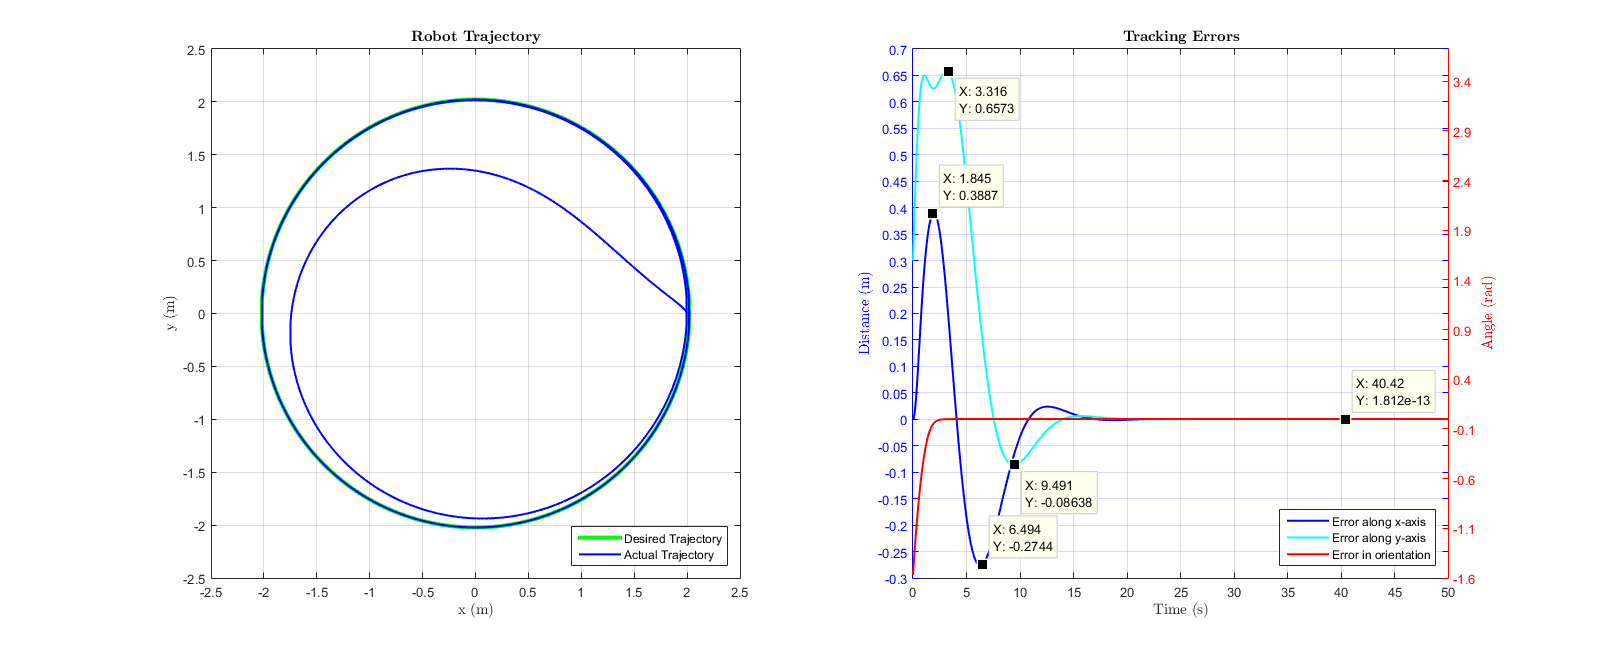
\includegraphics[width = 0.8\textwidth]{Figures/figure3.png}
\caption{Robot Trajectory and errors in $R_{0}$ frame with $K_{x}=1$, $K_{y}=1$ and $K_{\theta}=1$ }
\label{fig:figure3}
\end{figure}
\begin{figure}[H]
\centering
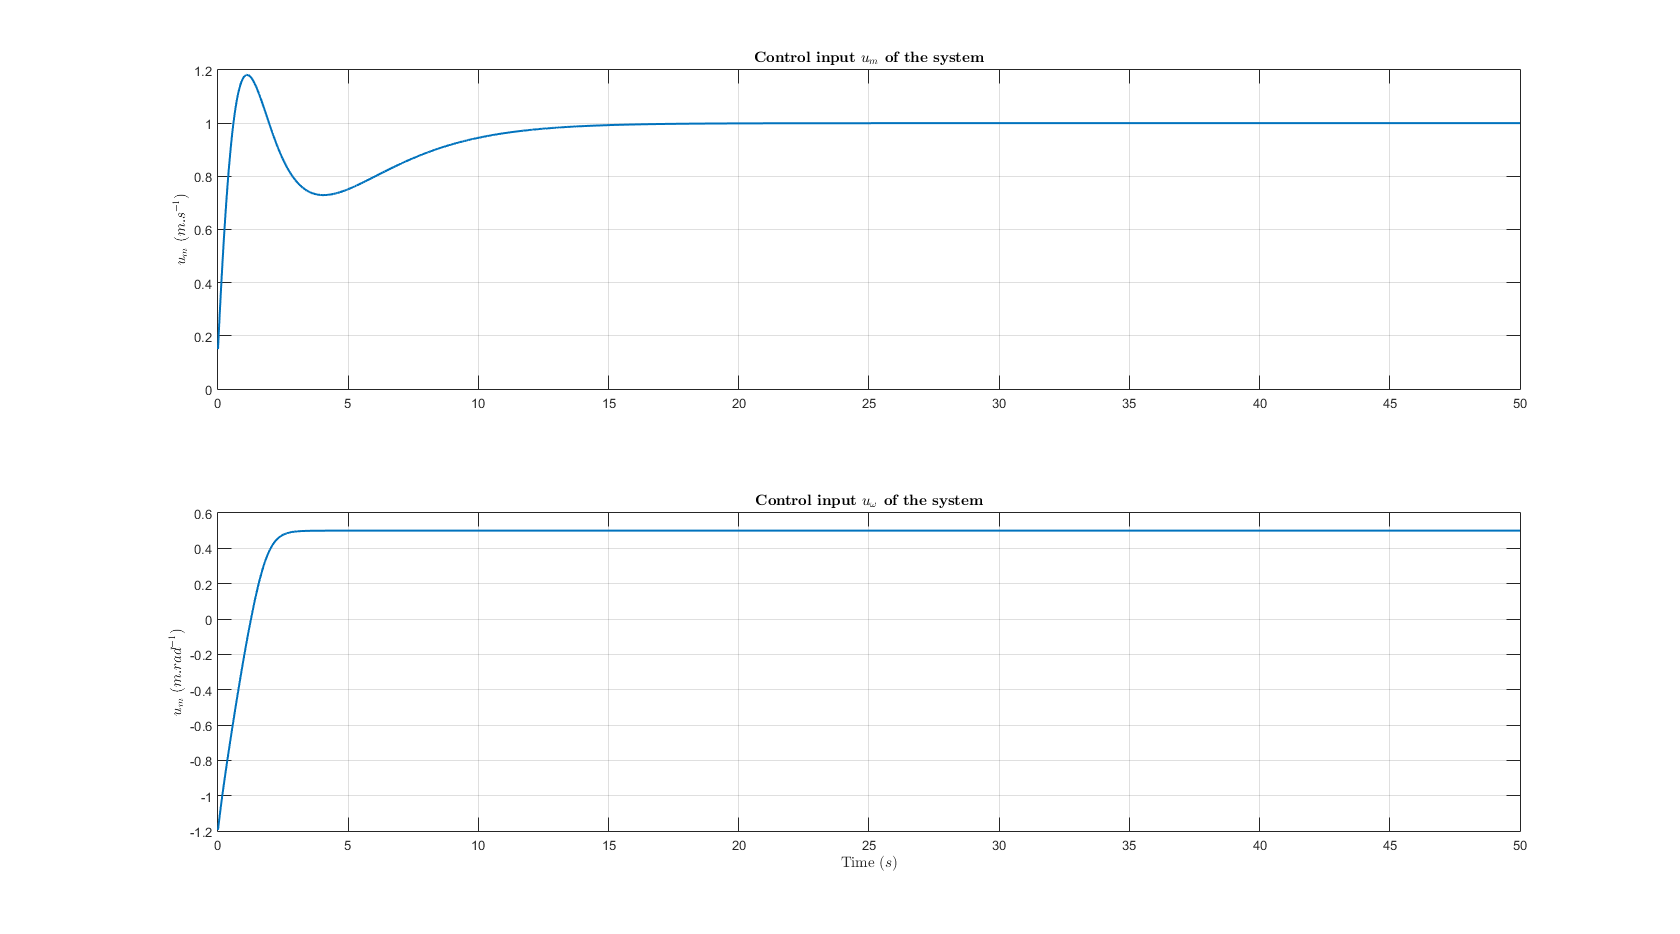
\includegraphics[width = 0.8\textwidth]{Figures/figure4.png}
\caption{Control inputs with $K_{x}=1$, $K_{y}=1$ and $K_{\theta}=1$ }
\label{fig:figure4}
\end{figure}
With these gains, the settling time is high and the transients are more pronounced (Figure \ref{fig:figure3}). This is evident from the high overshoots and undershoots in errors of both $x$ and $y$ axes, but error in $\theta$ goes to zero rapidly. Though all the errors settle down to zero after approximately 15 seconds, increasing the gain may reduce the transients. 
\item Tuning with $K_{x}=1$, $K_{y}=5$ and $K_{\theta}=6$: 
\begin{figure}[H]
\centering
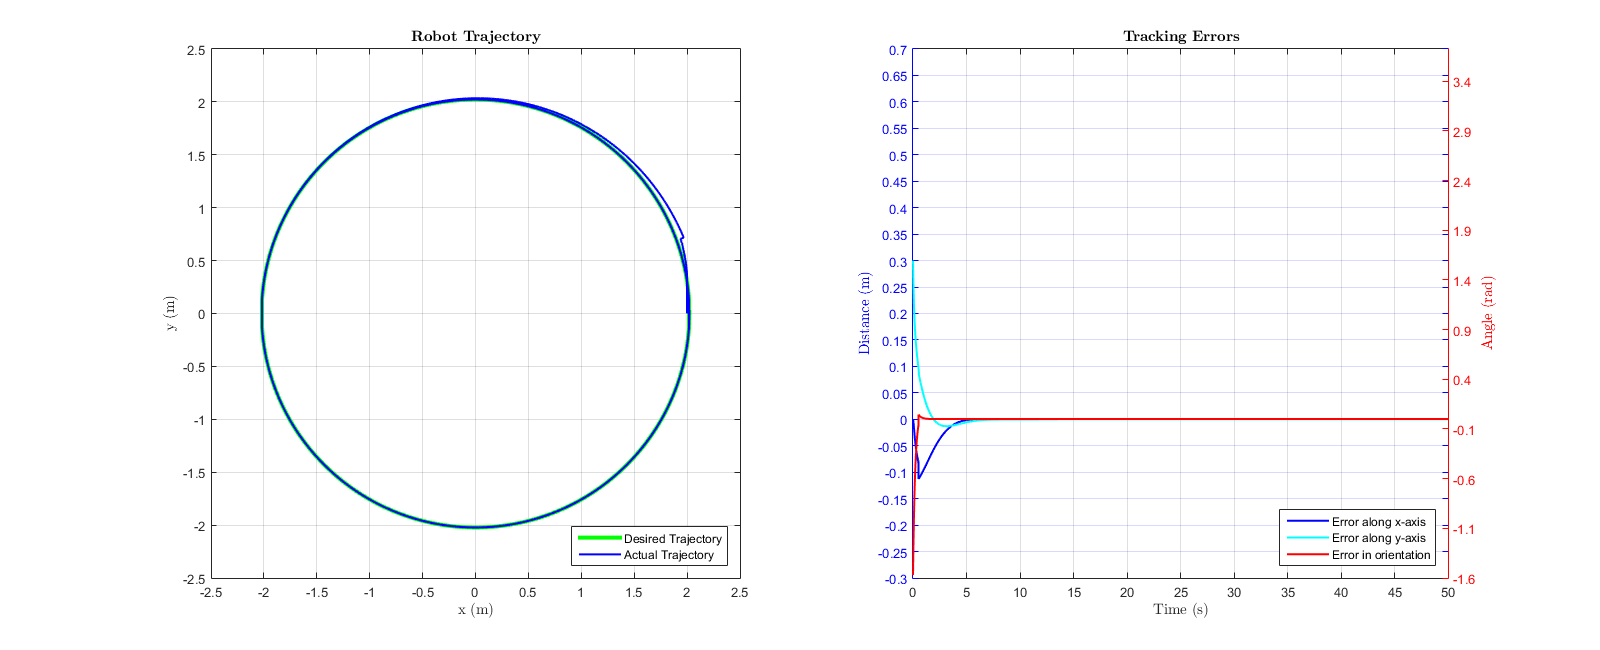
\includegraphics[width = 0.8\textwidth]{Figures/figure5.png}
\caption{Robot Trajectory and errors in $R_{0}$ frame with $K_{x}=1$, $K_{y}=5$ and $K_{\theta}=6$ }
\label{fig:figure5}
\end{figure}
\begin{figure}[H]
\centering
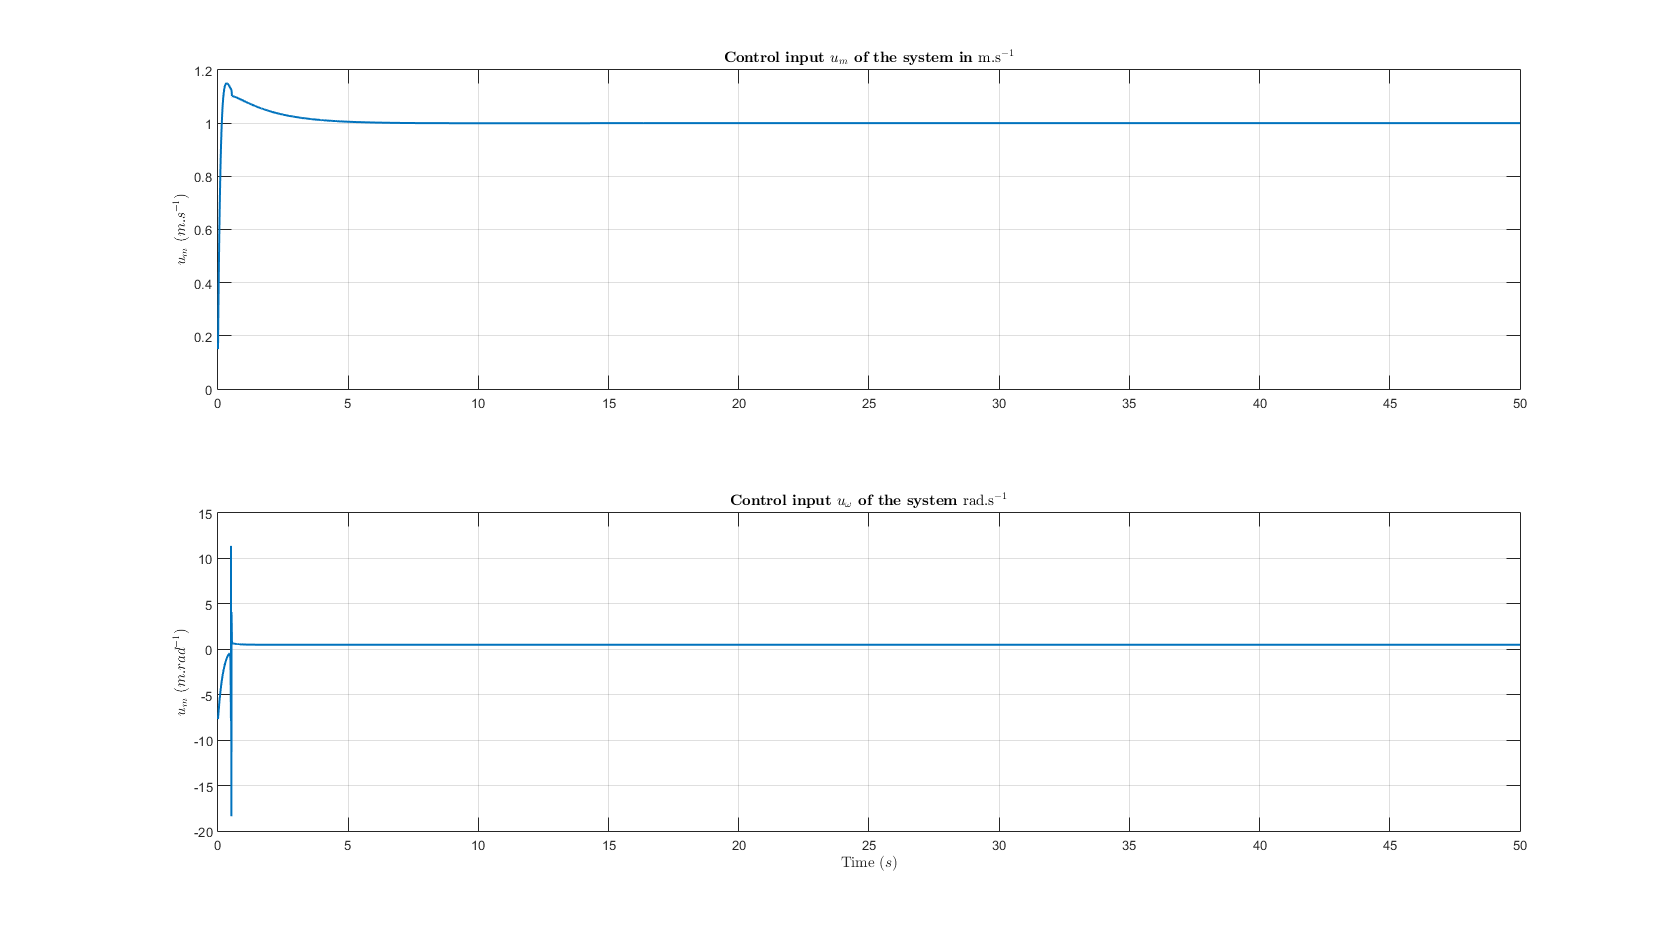
\includegraphics[width = 0.8\textwidth]{Figures/figure6.png}
\caption{Control inputs with $K_{x}=1$, $K_{y}=5$ and $K_{\theta}=6$ }
\label{fig:figure6}
\end{figure}
In Figure \ref{fig:figure5} the effect of increased gains is presented. The settling time has reduced significantly and the undershoots and overshoots (the transients) are less pronounced. All the errors converge to zero in approximately 7 seconds. In Figure \ref{fig:figure6} the control signals for these gains are presented. As the gain is higher, the control input during 0.45 to 0.53 seconds is a little aggressive but this in practice will not affect a mechanical system due to its inertia. 
\end{itemize}
\textbf{Effect of Parameter Variation}
\begin{itemize}
\item \textbf{Case 1:} 10\% increase in value of \textbf{a} only
\begin{figure}[H]
\centering
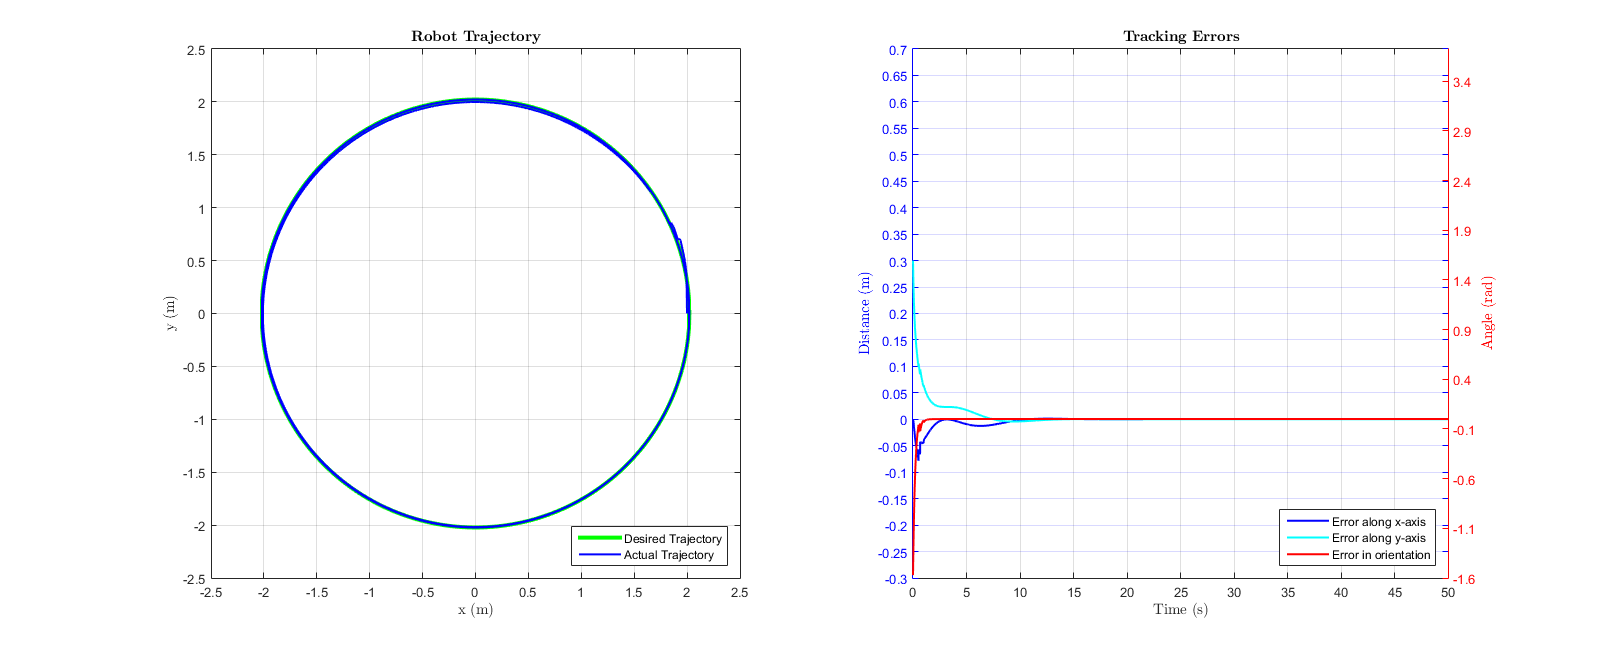
\includegraphics[width = 0.8\textwidth]{Figures/figure7.png}
\caption{Robot Trajectory and errors in $R_{0}$ frame with $K_{x}=1$, $K_{y}=5$ and $K_{\theta}=6$ and 10\% increase in value of a }
\label{fig:figure7}
\end{figure}

\begin{figure}[H]
\centering
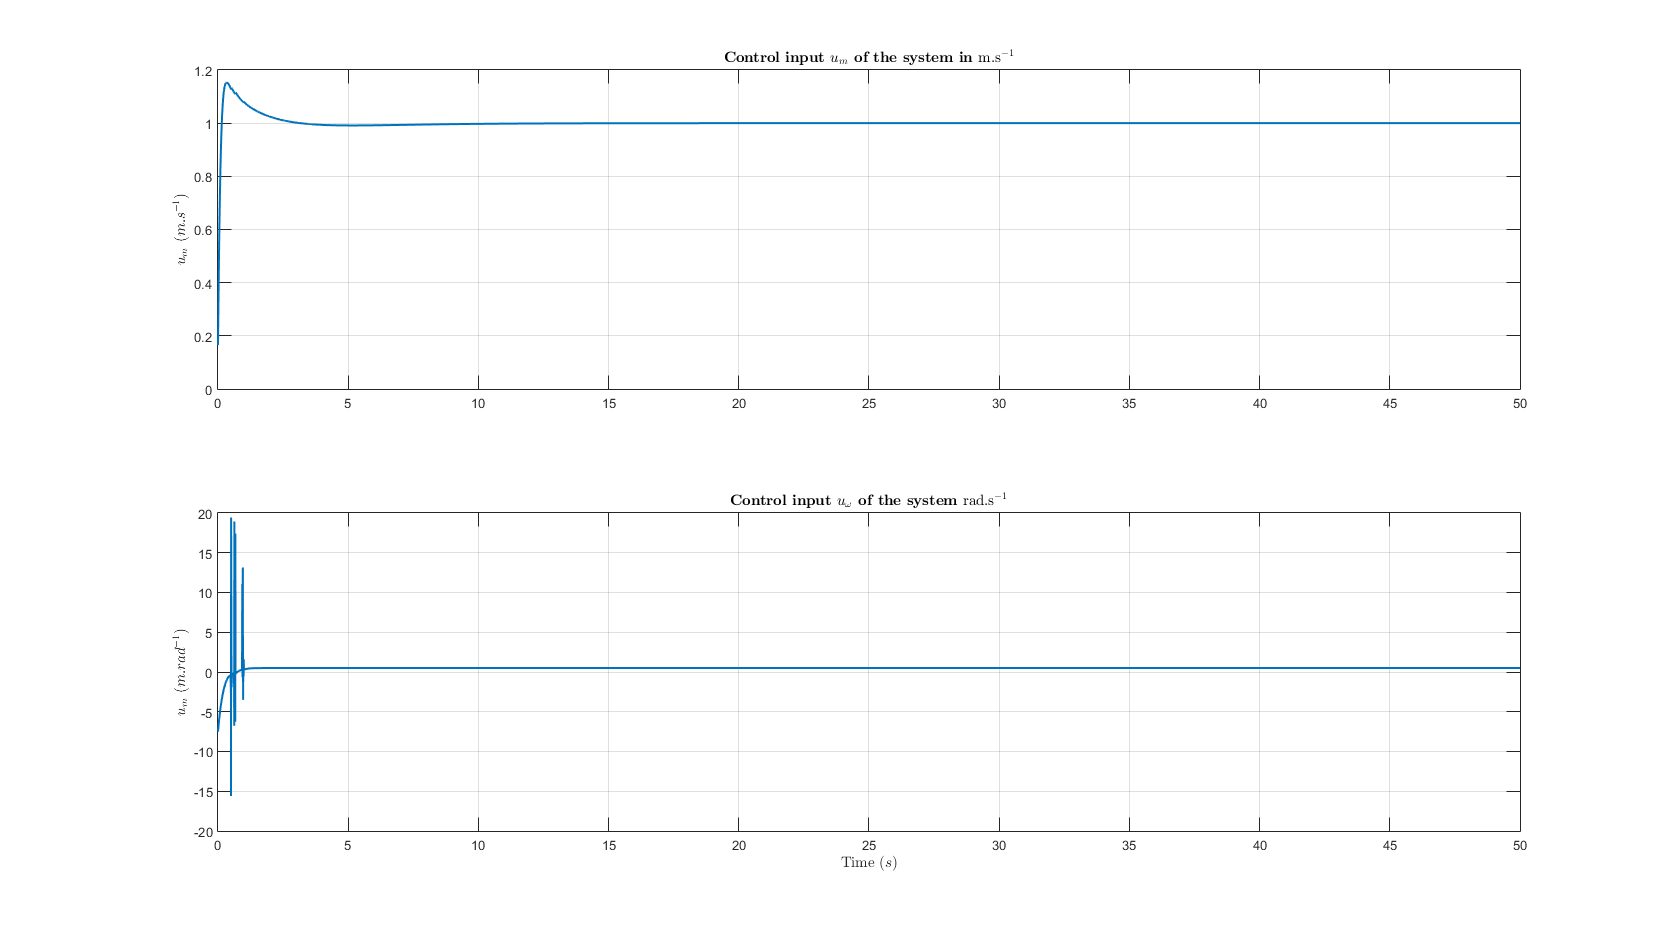
\includegraphics[width = 0.8\textwidth]{Figures/figure8.png}
\caption{Control inputs with $K_{x}=1$, $K_{y}=5$ and $K_{\theta}=6$ and 10\% increase in value of a }
\label{fig:figure8}
\end{figure}
In Figure \ref{fig:figure7} the effect of parameter variation can be observed, the settling time has increased (approximately 15 seconds)but all the errors go down to zero. In Figure \ref{fig:figure8} it can be seen that if the parameter changes a little then the control signal also changes, there is a lot of chatter in the value of $u_{\omega}$ in the first 1.5 seconds but gradually it settles down to the desired angular velocity of the vehicle. It is observed (Figure \ref{fig:figure9} and Figure \ref{fig:figure10}) that reducing $K_{y}$ and $K_{\theta}$ to $K_{y}=4$ and $K_{\theta}=5$ removes all the rapid fluctuations in value of $u_{\omega}$ but there is no significant change in the settling time, nevertheless, all the errors converge to zero eventually.

\begin{figure}[H]
\centering
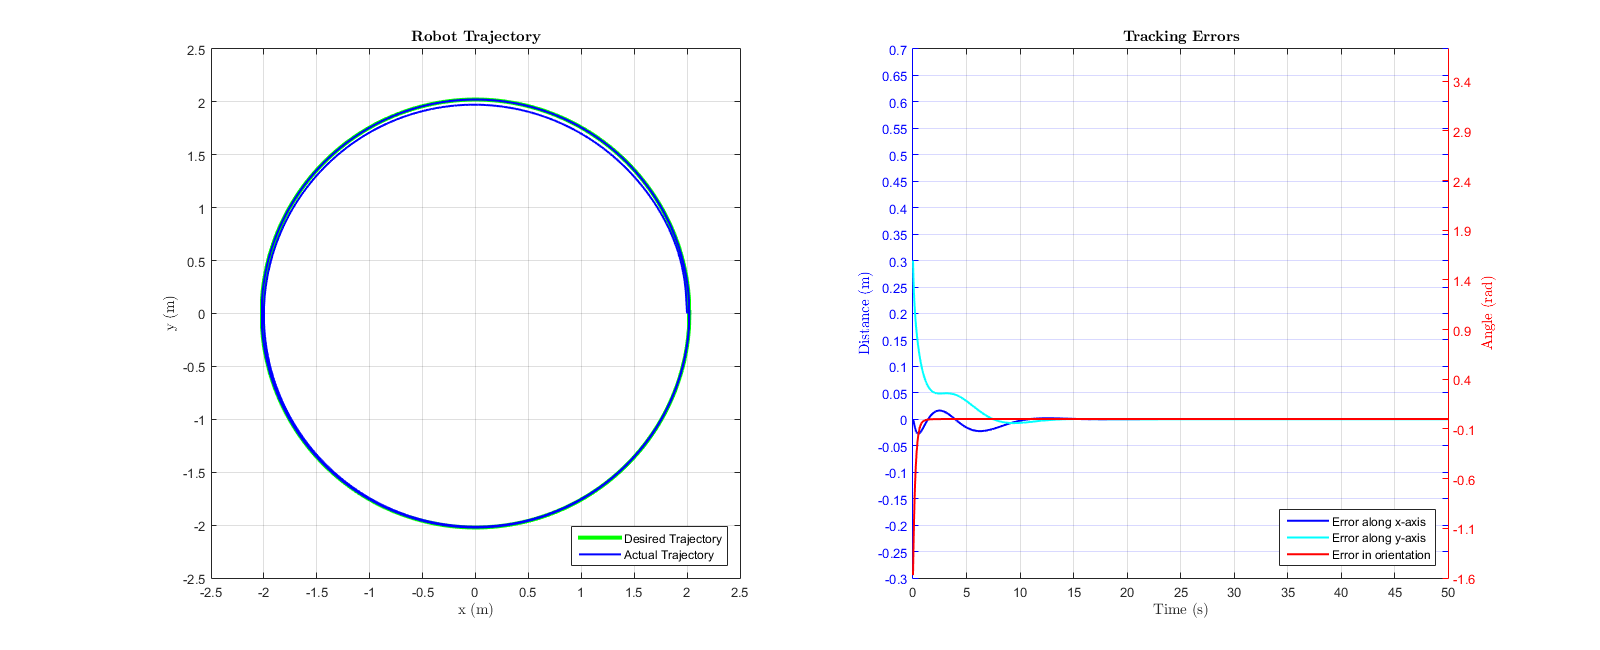
\includegraphics[width = 0.8\textwidth]{Figures/figure9.png}
\caption{Robot Trajectory and errors in $R_{0}$ frame with $K_{x}=1$, $K_{y}=4$ and $K_{\theta}=5$ and 10\% increase in value of a }
\label{fig:figure9}
\end{figure}

\begin{figure}[H]
\centering
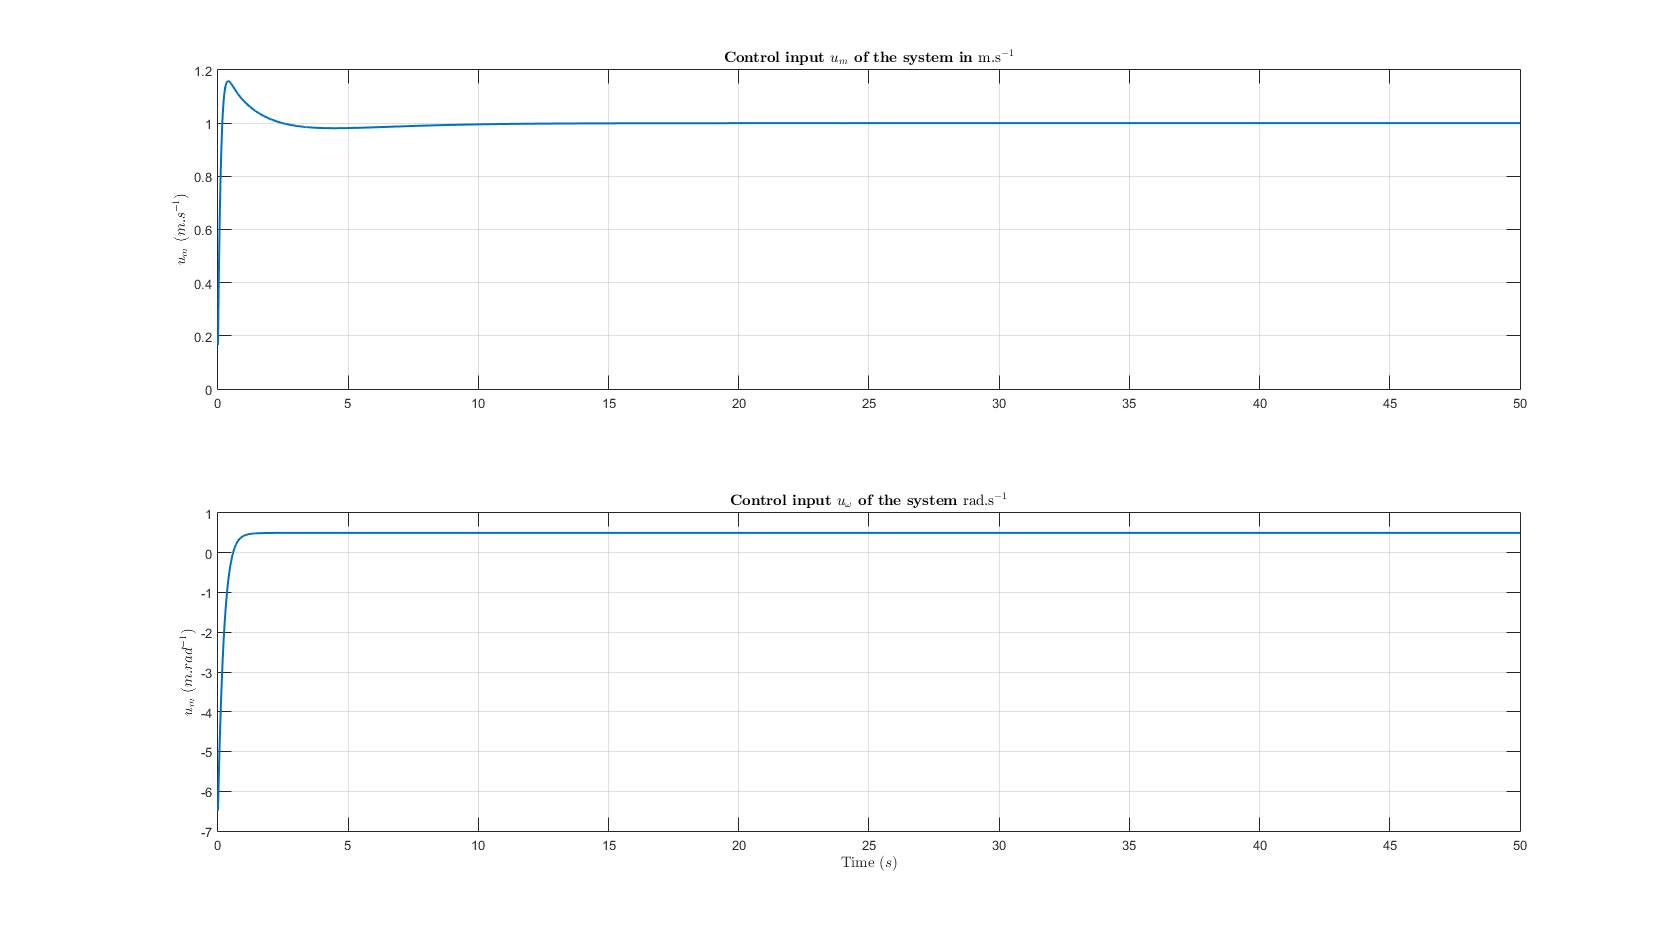
\includegraphics[width = 0.8\textwidth]{Figures/figure10.png}
\caption{Control inputs with $K_{x}=1$, $K_{y}=4$ and $K_{\theta}=5$ and 10\% increase in value of a }
\label{fig:figure10}
\end{figure}

\item \textbf{Case 2:} 10\% increase in value of \textbf{r} only
\begin{figure}[H]
\centering
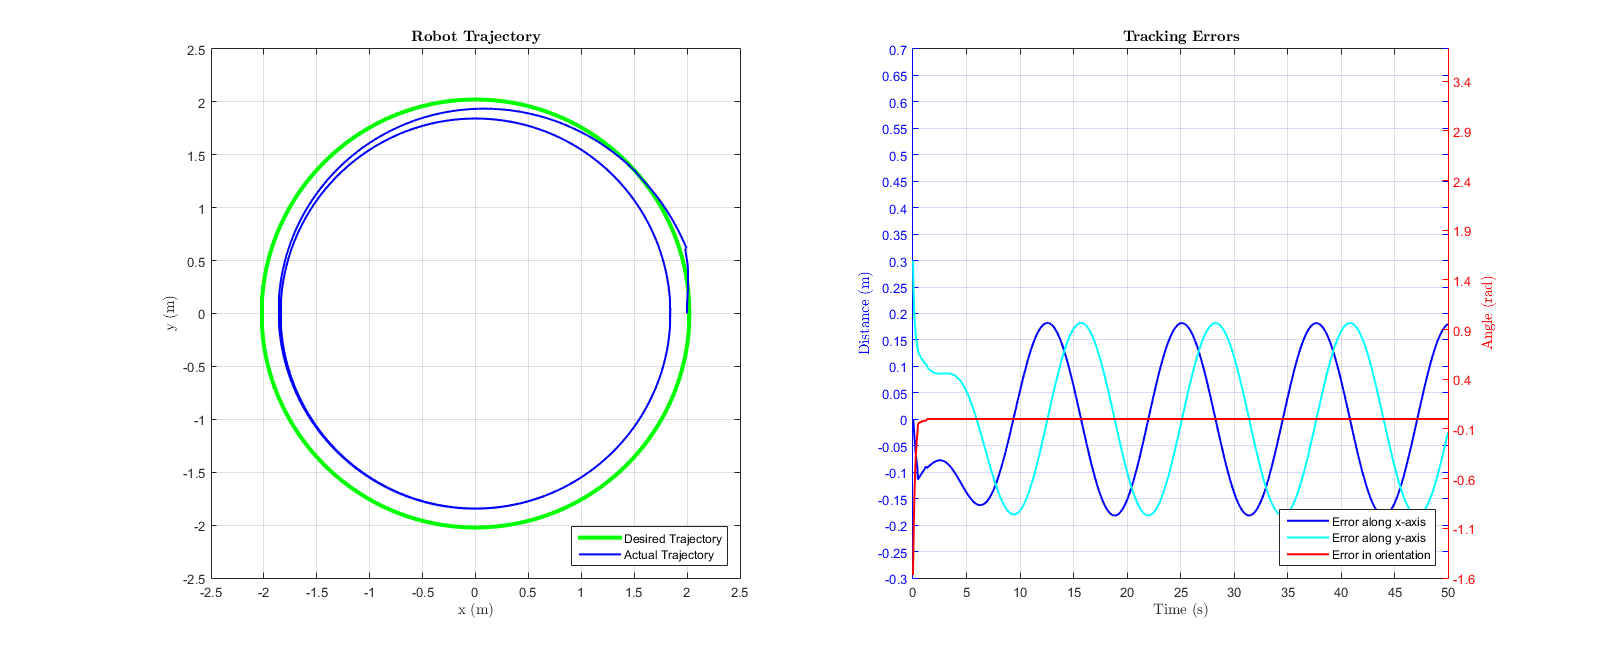
\includegraphics[width = 0.8\textwidth]{Figures/figure11.png}
\caption{Robot Trajectory and errors in $R_{0}$ frame with $K_{x}=1$, $K_{y}=5$ and $K_{\theta}=6$ and 10\% increase in value of r }
\label{fig:figure11}
\end{figure}

\begin{figure}[H]
\centering
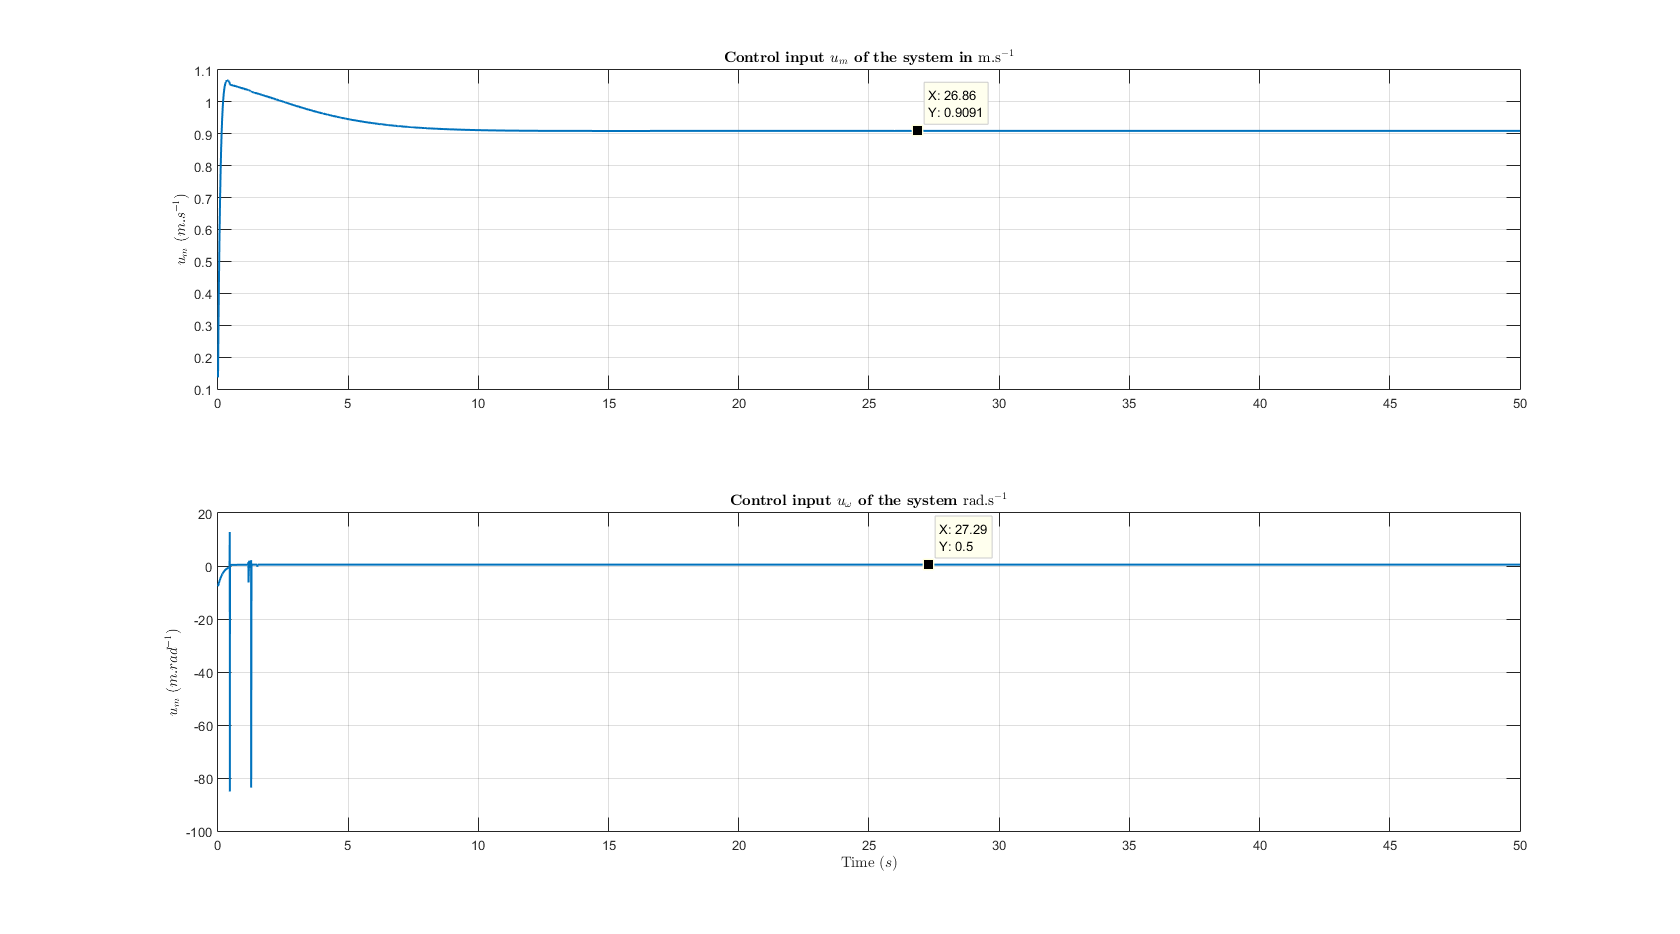
\includegraphics[width = 0.8\textwidth]{Figures/figure12.png}
\caption{Control inputs with $K_{x}=1$, $K_{y}=5$ and $K_{\theta}=6$ and 10\% increase in value of r }
\label{fig:figure12}
\end{figure}

In Figures \ref{fig:figure11} and \ref{fig:figure12} the effect of variation of the wheel radius r is seen. The effects are severe. The trajectory converges to a path of radius smaller than the required radius, thus explaining the oscillating errors in global $x$ and $y$ coordiantes, but error in $\theta$ converges to zero.\\
For any reasonable value of gain we take, the trajectory will converges to the path of same radius as seen in Figure \ref{fig:figure11} and \ref{fig:figure13}   which is lesser than the required radius. 
\begin{figure}[H]
\centering
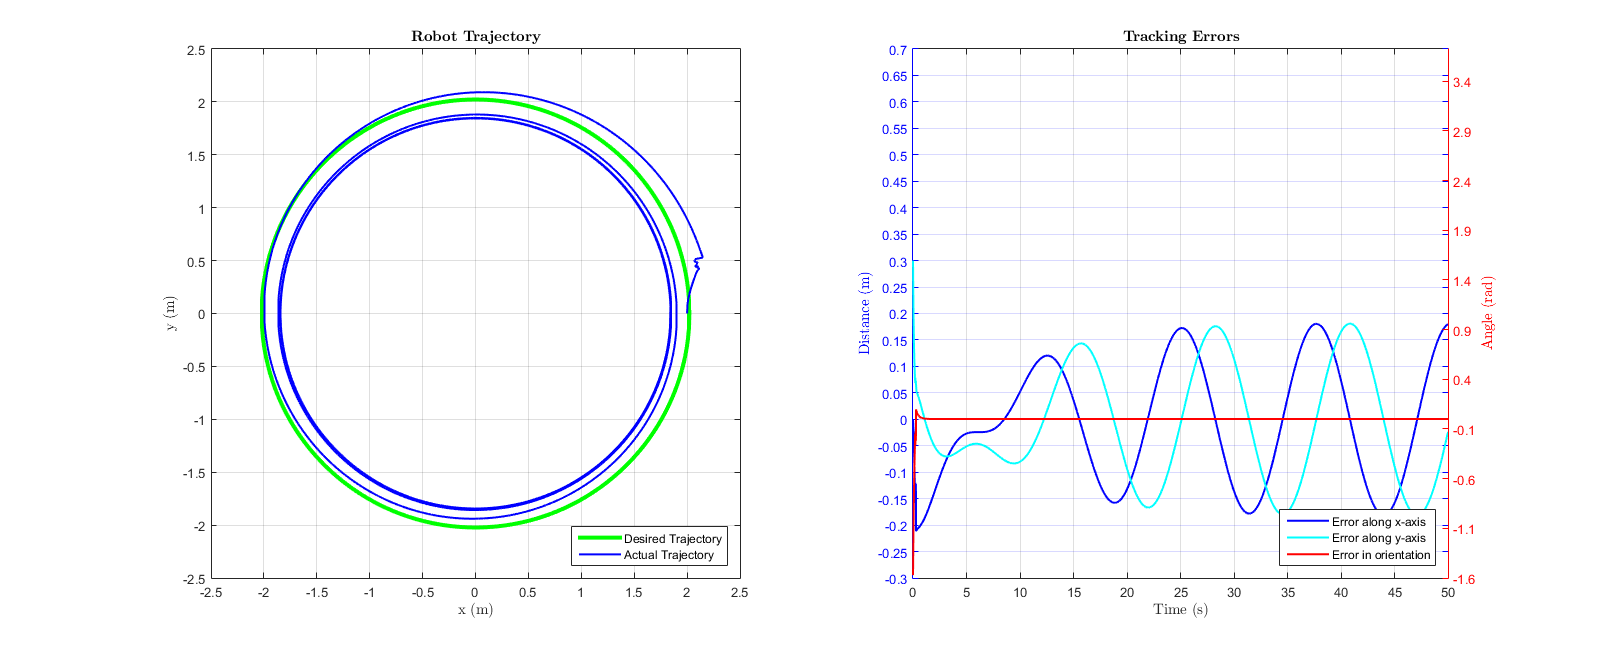
\includegraphics[width = 0.8\textwidth]{Figures/figure13.png}
\caption{Robot Trajectory and errors in $R_{0}$ frame with $K_{x}=2$, $K_{y}=5$ and $K_{\theta}=10$ and 10\% increase in value of r }
\label{fig:figure13}
\end{figure}

\begin{figure}[H]
\centering
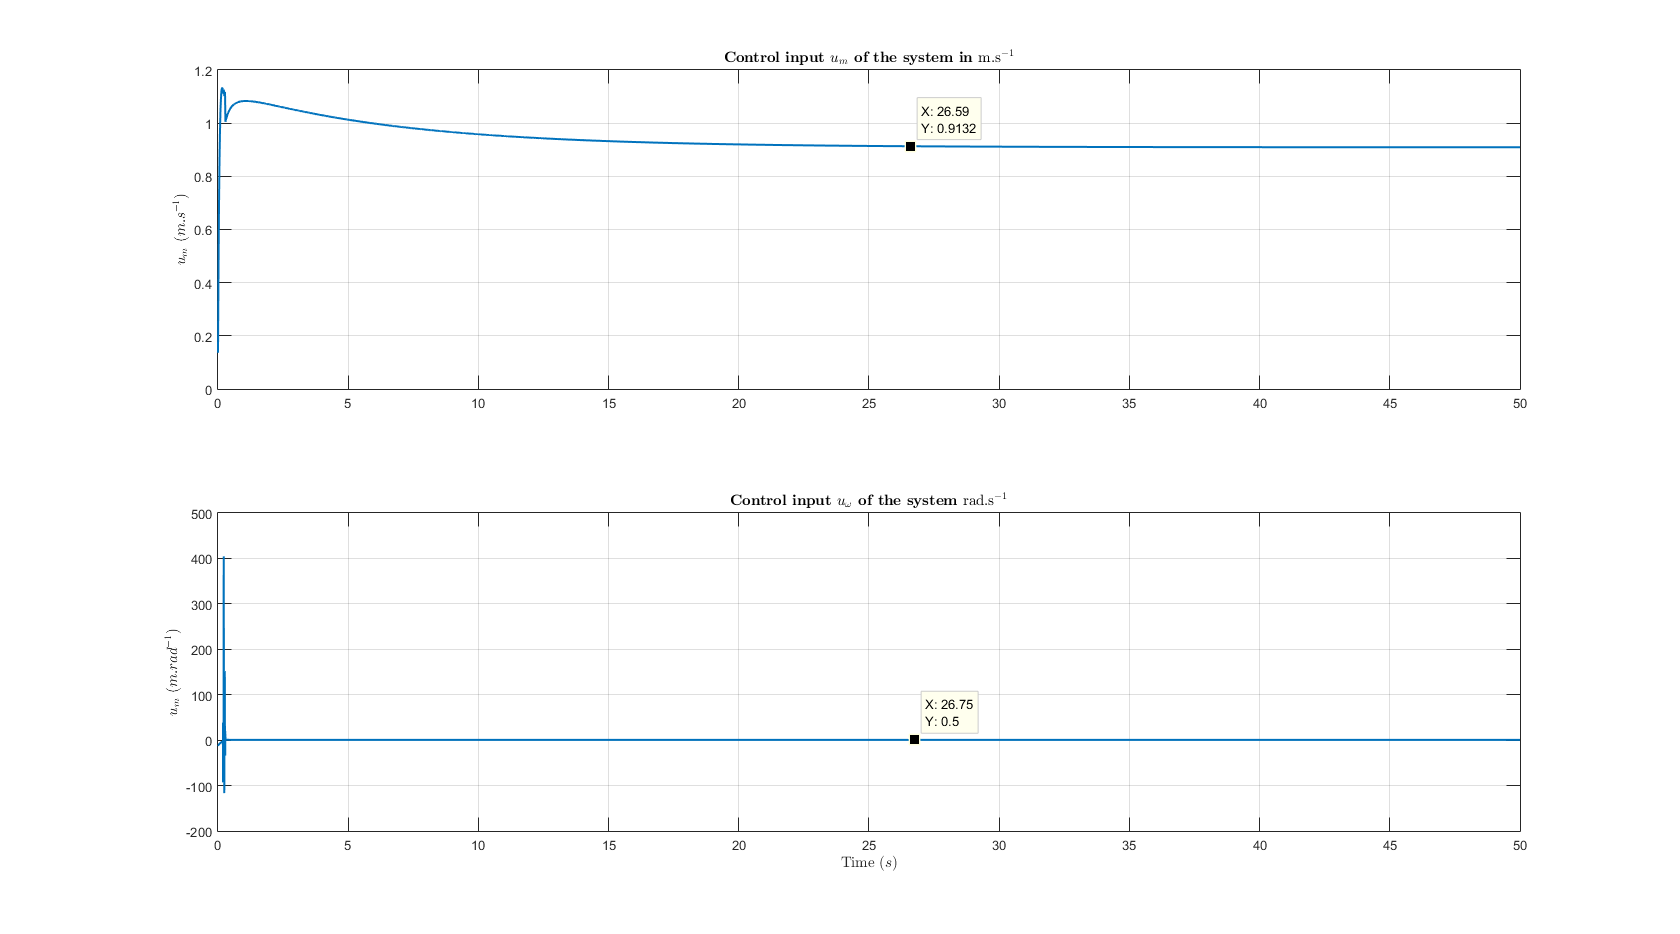
\includegraphics[width = 0.8\textwidth]{Figures/figure14.png}
\caption{Control inputs with $K_{x}=2$, $K_{y}=5$ and $K_{\theta}=10$ and 10\% increase in value of r }
\label{fig:figure14}
\end{figure}
The cause can be found in Figure \ref{fig:figure12} and \ref{fig:figure14} . The translational velocity $u_m$ converges to 0.9 $m.s^{-1}$ approximately (lesser than 1 $m.s^{-1}$, the reference translational velocity )and the angular velocity converges to 0.5 $rad.s^{-1}$ (equal to the reference angular velocity), using these values the radius of the path obtained is $r=\frac{0.9}{0.5}=1.8$ metres (less than the desired radius). This effect of parameter variation is not mitigated even on increasing the gains, a solution could be to add an error term to the control output $u_m$, doing so will account for the difference in $u_{mr}$(the required $u_m$) and the actual $u_m$ under parameter variation.\\


\begin{figure}[H]
\centering
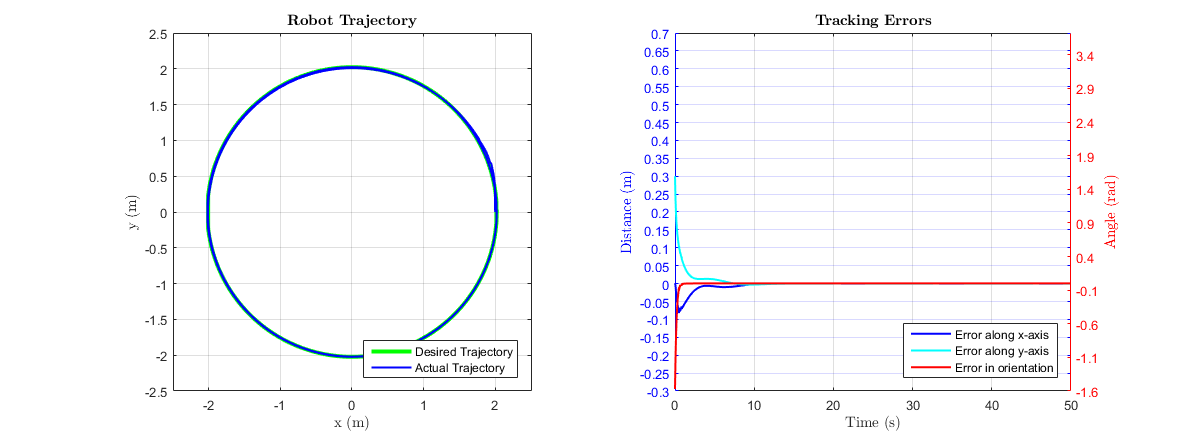
\includegraphics[width = 0.8\textwidth]{Figures/figure15.png}
\caption{Robot Trajectory and errors in $R_{0}$ frame with $K_{x}=1$, $K_{y}=5$ and $K_{\theta}=6$ and 10\% increase in value of r }
\label{fig:figure15}
\end{figure}

\begin{figure}[H]
\centering
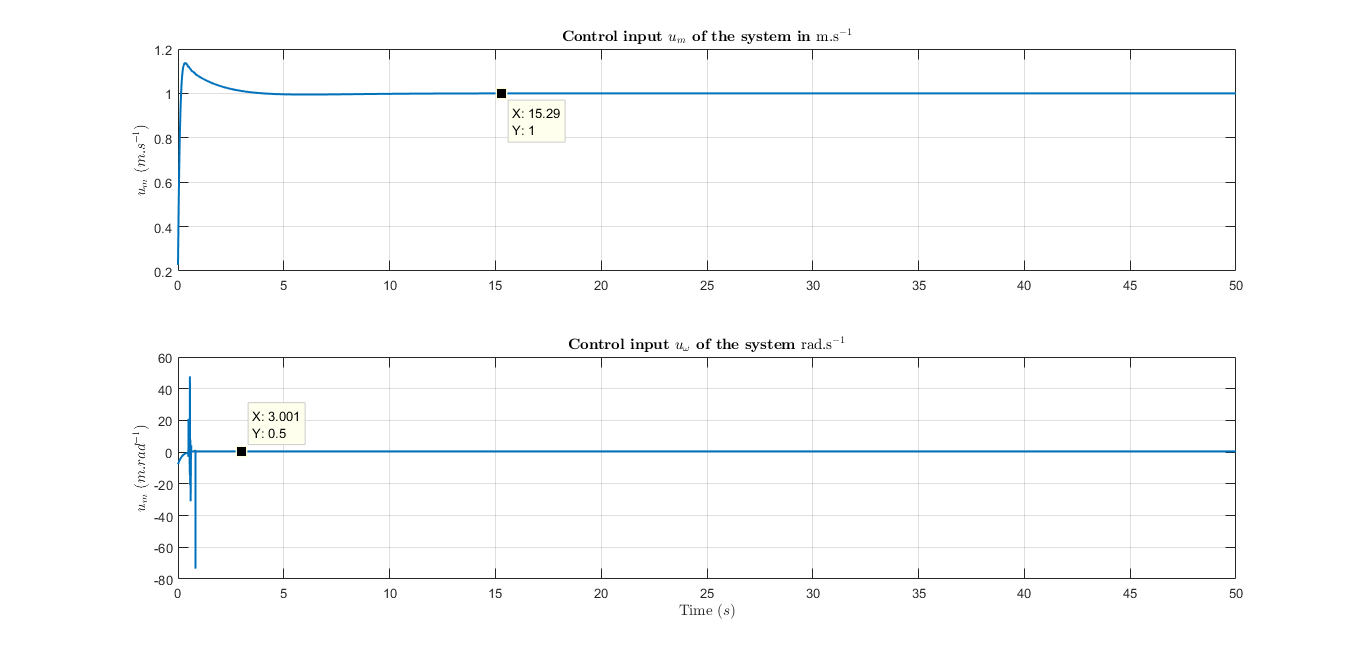
\includegraphics[width = 0.8\textwidth]{Figures/figure16.png}
\caption{Control inputs with $K_{x}=1$, $K_{y}=5$ and $K_{\theta}=6$ and 10\% increase in value of r }
\label{fig:figure16}
\end{figure}

The effect of adding $u_{mr}-u_{m}$(=$1-0.9=0.1$ for this case) to the controller output $u_m$ is seen in Figure \ref{fig:figure15} and \ref{fig:figure16}. Clearly, the response improves drastically. Thus the effect of parameter variation in this case can be mitigated by adding the error in the required control output and the actual control output.
\end{itemize}

\end{document}